\chapter{Literature Review}

This chapter presents some milestones in the history of autonomous driving and also some of the most relevant projects made previously in the ATLASCAR2. It also presents examples of \gls{adas} datasets for labelled data.


\section{Milestones on the History of autonomous driving}

Overall, motorized road transport led to the accidental deaths of around 200,000 US citizens in the 1920s; by far the greatest number of these were pedestrians (\cite{Kroger2016}). The idea of substituting error-prone humans with technology thus practically suggested itself. The first registered experiments for \gls{ad} have been conducted circa the 1920's (\cite{TheMilwaukeeSentinel}) in Milwaukee (see figure \ref{fig:phantomauto}). A 1926 Chandler was equipped with a transmitting antennae and was radio-controlled by a second car that followed it.

\begin{figure}[htp]
	
	\centering
	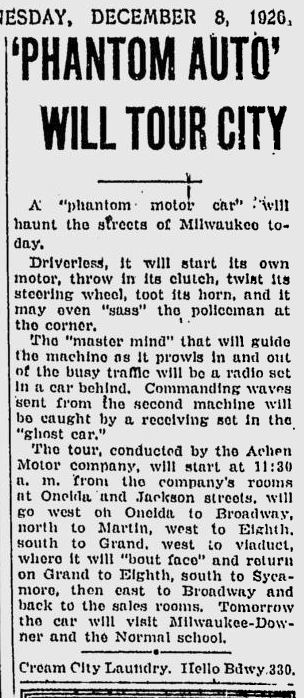
\includegraphics[width=0.25\textwidth]{capstate/imgs/jornal.png}
	
	\caption{\cite{TheMilwaukeeSentinel}, 8 December - 'Phantom Auto' Will Tour City}
	\label{fig:phantomauto}
	
\end{figure}

In the 1950s promising trials in \gls{ad} took place. General Motors conducted experiments in miniature models along with the electronic manufacturer \gls{rca}. The two companies later developed a full size system that was successfully demonstrated completing a test route of one mile (\cite{Kroger2016}).

In the 1980s, pioneer Ernst Dickmanns designed a vision-guided Mercedes Benz along with the Bundeswehr University Munich engineering team, achieving a speed of 63 km/h on streets with no traffic. In the late 80s, projects with both \gls{lidar} scanners and computer vision were carried out. In 1989 the first experiments with vehicles making use of neural networks were conducted (\cite{Pomerleau1989}).

Various autonomous vehicles competitions have been held. The first long distance competition for driverless cars was the \gls{darpa} Grand Challenge (\cite{DARPA}). The event was open to teams and organizations from around the world. Teams have participated from high schools, universities, businesses and other organizations, bringing a wide variety of technological skills to the race. The challenge offered high value money prizes to the winners. Because the reward was so high, the contest brought various state-of-the-art autonomous vehicles that showcased the solutions implemented in the platforms featuring new ideas that used the most recent technologies (\cite{Montemerlo2006} and \cite{Thrun2007}).

Since then, many companies and research organizations have been developing various prototype cars. In the past decade, electric motored cars have emerged and new opportunities for \gls{ad} and \gls{adas} research have appeared. 

Waymo, the Google self-driving car project, begun testing driverless cars without someone at the driver position. The Waymo project started in 2009 and it counts more than 5 million miles self-driven. Google has recently partnered with Jaguar and designed self-driving Jaguar I-PACEs (figure \ref{fig:waymo}). Tests on the newest self-driving Waymo's vehicle will be conducted in 2018 (\cite{Waymo}).


\begin{figure}[htp]
	
	\centering
	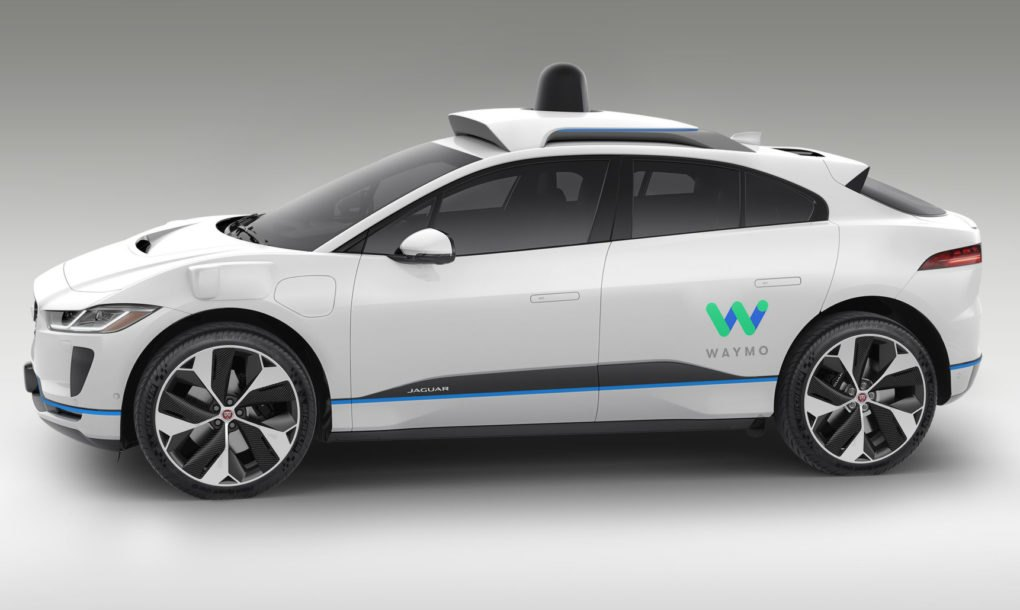
\includegraphics[width=0.9\textwidth]{capstate/imgs/waymo}
	
	\caption{Waymo's Jaguar I-PACE \cite{Waymo}}
		\label{fig:waymo}
	
\end{figure}

Another example of an autonomous vehicle project is the Uber \gls{atc} car based on an hybrid Ford Fusion (figure \ref{fig:uber}). The vehicle is equipped with state of the art \gls{lidar} scanners, and several vision-based sensors and radars.

\begin{figure}[htp]
	
	\centering
	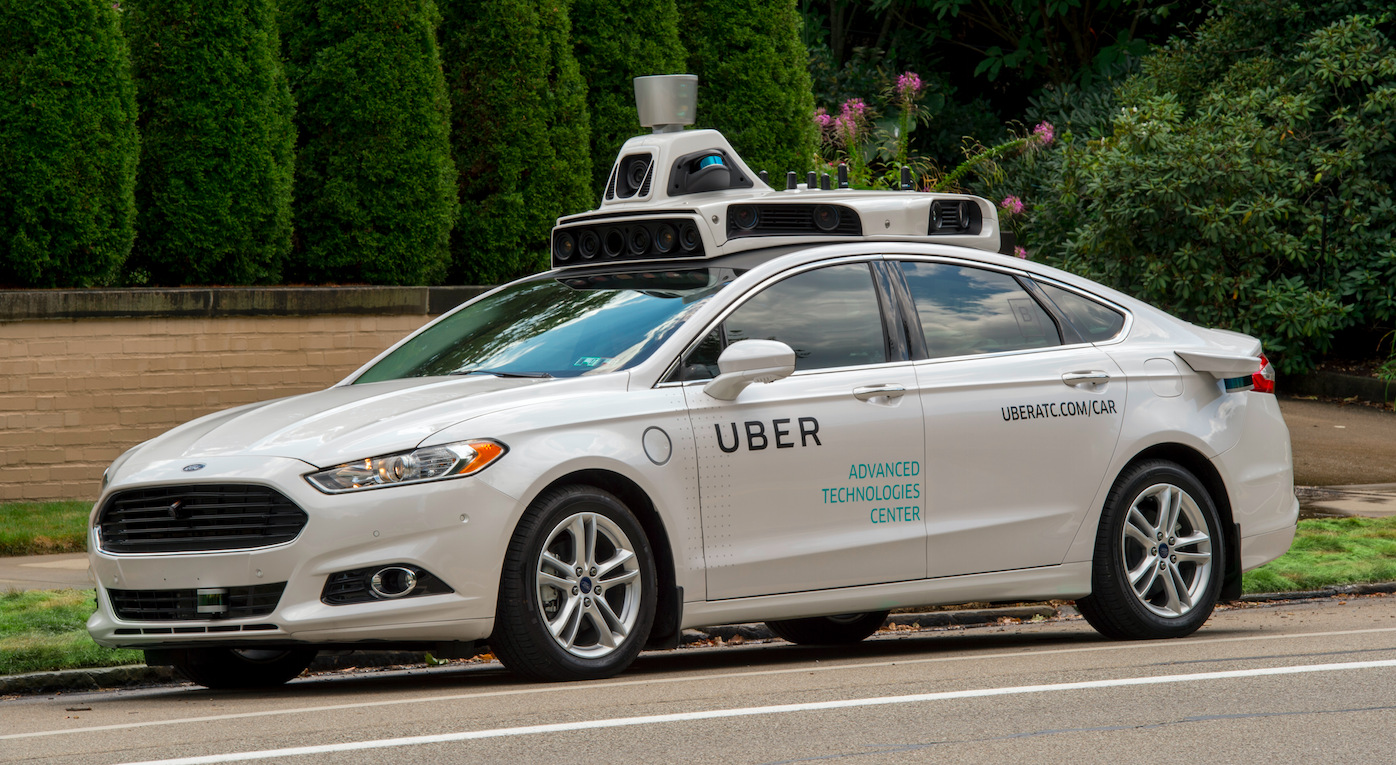
\includegraphics[width=0.9\textwidth]{capstate/imgs/uber}
	
	\caption{Ford Fusion Uber ATC car (\cite{UberAdvancedTechnologiesGroup})}
	\label{fig:uber}
	
\end{figure}

Audi released its A8 (figure \ref{fig:audi}) and the company stated that they would be the first manufacturer to use laser scanners in addition to cameras and others sensors in autonomous vehicles. The vehicle was designed to a level 3 autonomous driving: it is capable of self-driving with the expectation that the human driver will respond appropriately to a request to intervene. The Audi AI traffic jam pilot takes over the driving task in slow-moving traffic up to 60 km/h (\cite{AudiMediaCenter} and \cite{AndreasHerrmannWalterBrenner2018}).

\begin{figure}[htp]
	
	\centering
	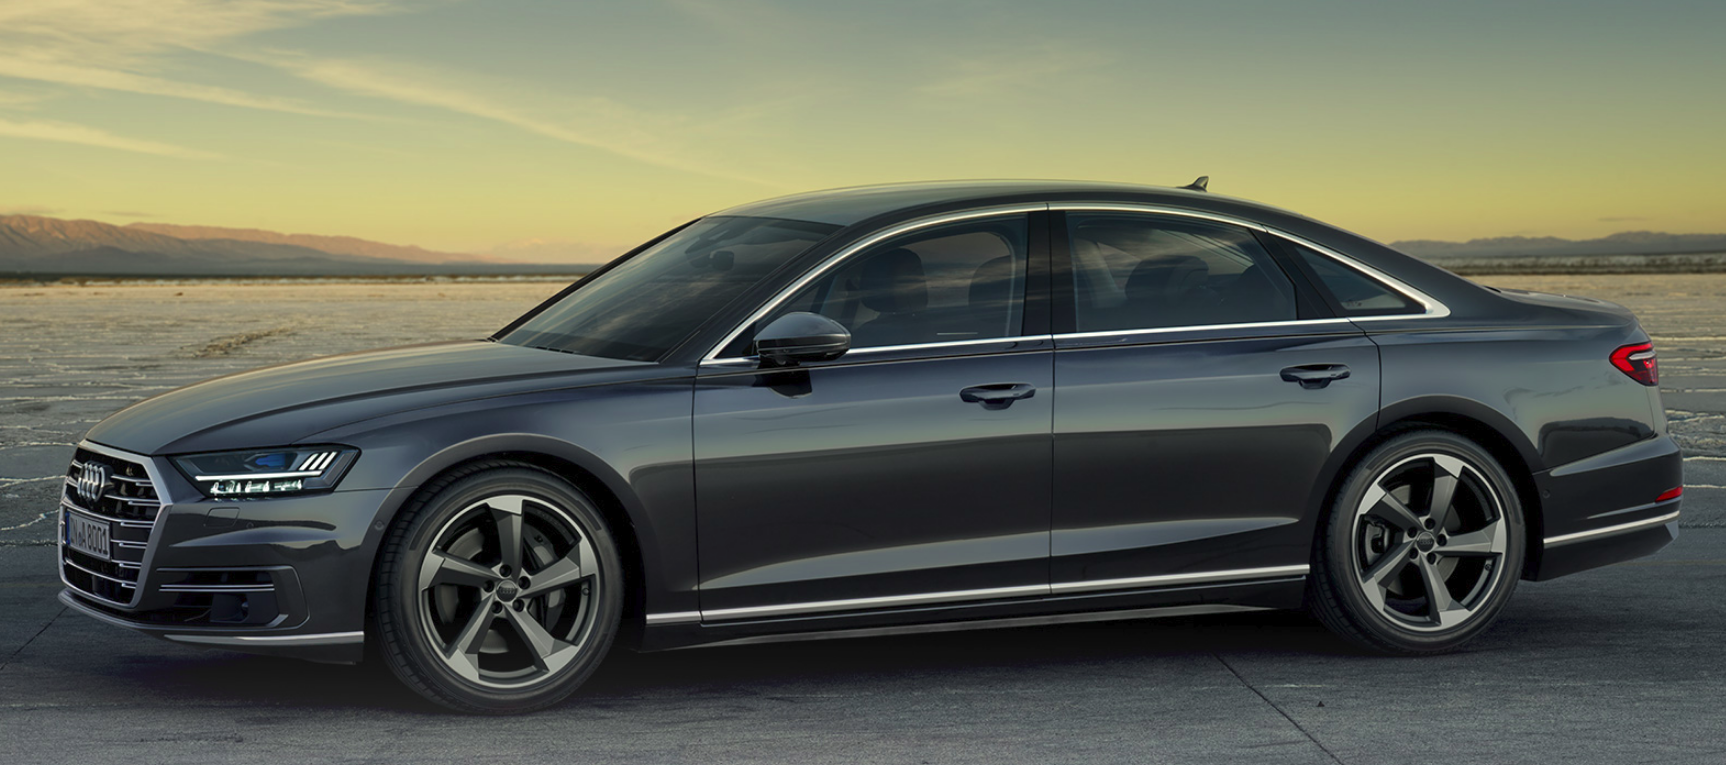
\includegraphics[width=0.9\textwidth]{capstate/imgs/audi}
	
	\caption{The new Audi A8 (\cite{AudiMediaCenter})}
	\label{fig:audi}
	
\end{figure}

Like the University of Aveiro, many other universities and research institutes study the \gls{ad} and \gls{adas} paradigms.

Another interesting autonomous vehicle project is the \gls{scot} vehicle (figure \ref{fig:scot}), conducted by the \gls{smart} (\cite{Singapore-MITAllianceforResearchandTechnology}). Like the ATLASCAR 2, \gls{scot} is also a Mitsubishi i-MiEV used to research \gls{adas} and \gls{ad} at \gls{smart} and it is designed for operations on public roads (\cite{AndreasHerrmannWalterBrenner2018}). The \gls{scot} vehicle also relies on \gls{lidar} sensors similar to ATLASCAR 2 (\cite{Teo}). 

\begin{figure}[htp]
	
	\centering
	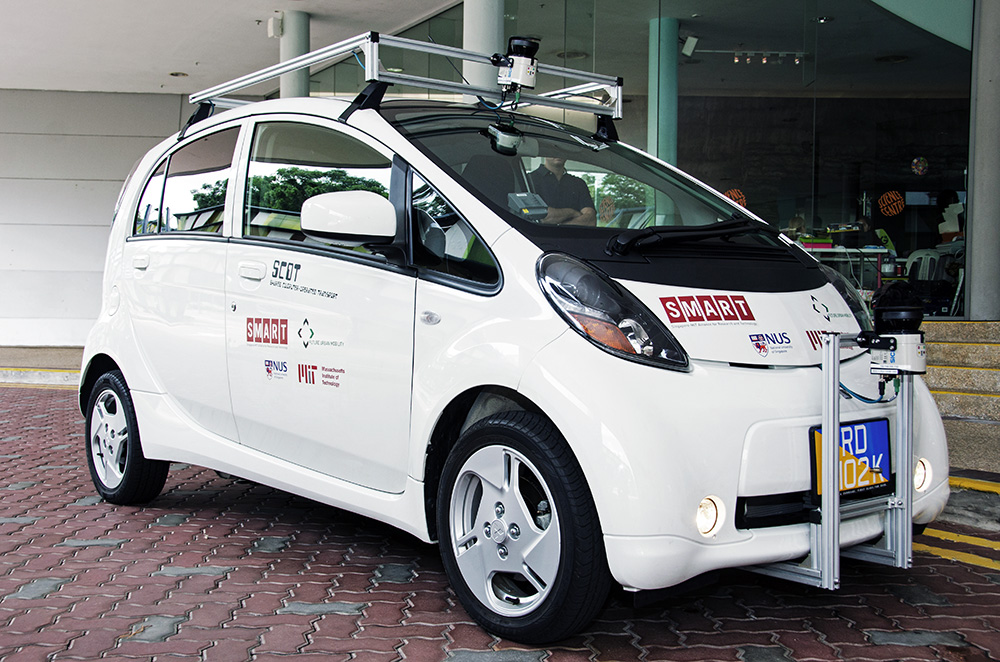
\includegraphics[width=0.9\textwidth]{capstate/imgs/scot}
	
	\caption{SCOT - Shared Computer-Operated Transit vehicle (\cite{Singapore-MITAllianceforResearchandTechnology})}
	\label{fig:scot}
	
\end{figure}

To resume this chapter, in figure \ref{fig:timeline} a timeline with the referred milestones is presented.

\begin{figure}[htp]
	
	\centering
	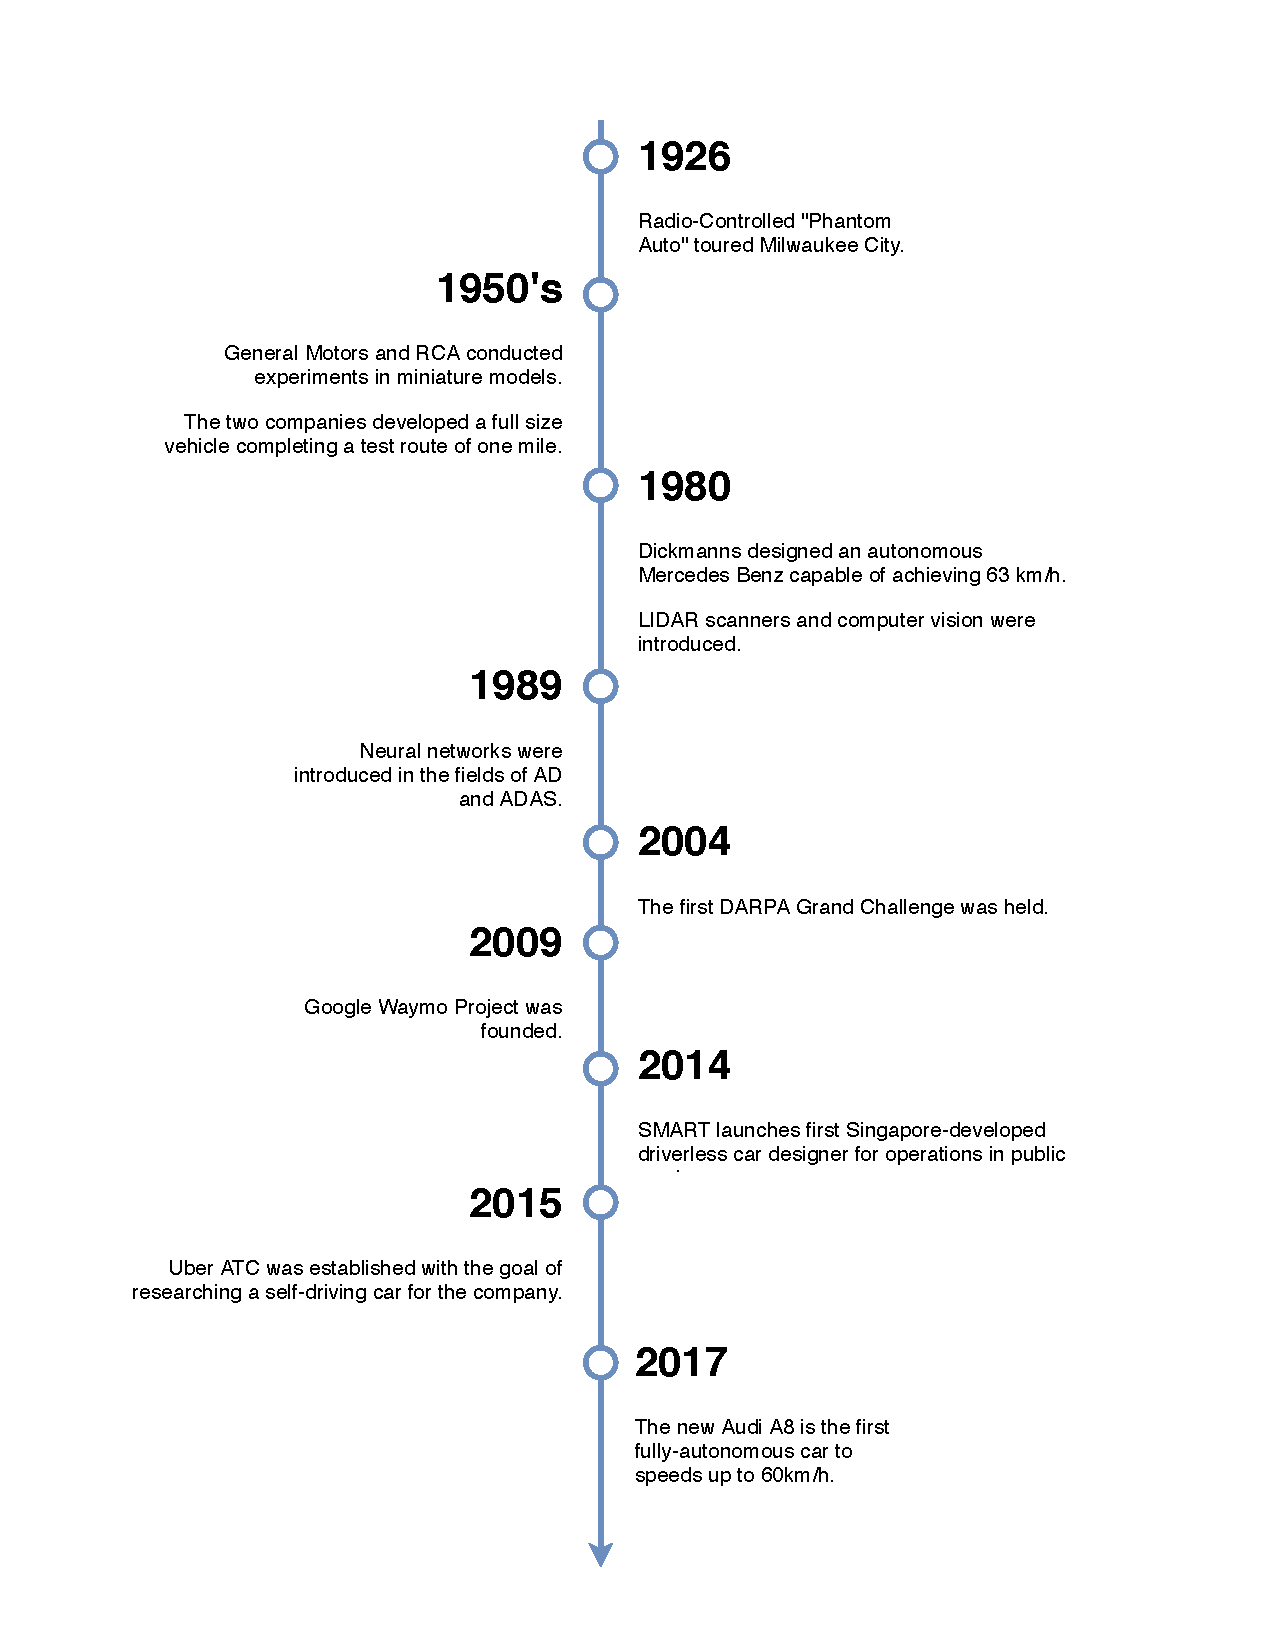
\includegraphics[width=1\textwidth]{capstate/imgs/timeline.pdf}
	
	\caption{Timeline with some milestone of autonomous driving history}
	\label{fig:timeline}
	
\end{figure}

\section{Related work on ATLASCAR2}

In this section it is referenced previous work done at \gls{lar} relevant for this thesis.

\subsection{Multisensor Calibration and Data Fusion Using LIDAR and Vision} 

The calibration procedure for data fusion of ATLASCAR was developed by \cite{VieiradaSilva2016}. The work presents an expansion to an existing extrinsic calibration package to vision-based sensors where a ball is used as calibration target. 

The calibration consists of a appearance-based algorithm to detect the ball in the image and a range-based algorithm to detect the ball in the surroundings. 

The calibration package consists in a graphical interface (see figure \ref{fig:david}) that allows the user to configure the various sensors to be calibrated. The estimated positions between sensors are achieved with sensor data fusion.

\begin{figure}[htp]
	
	\centering
	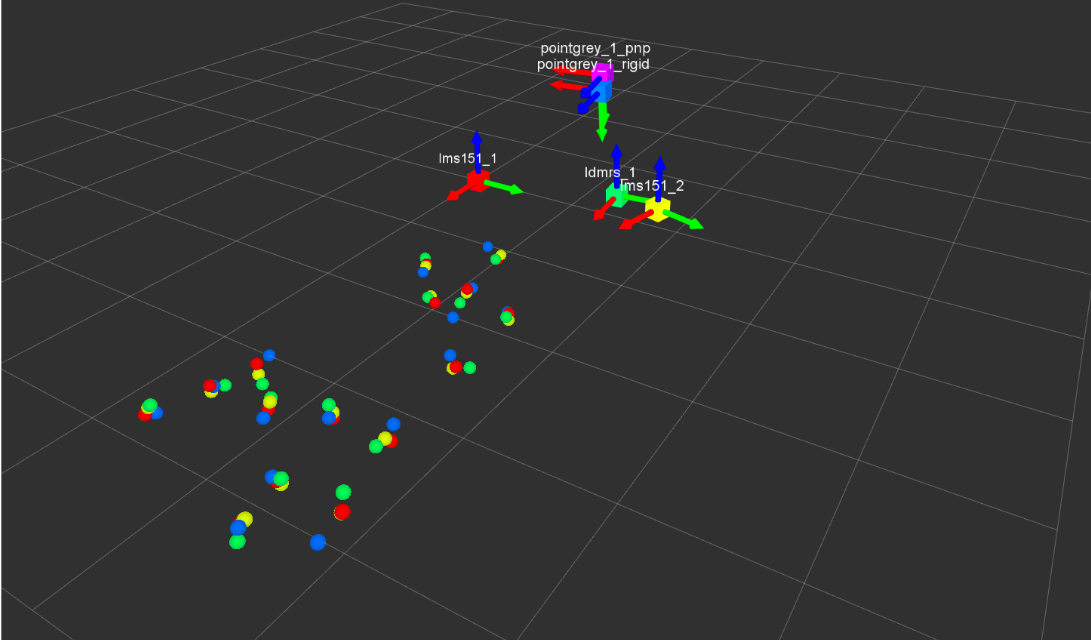
\includegraphics[width=1\textwidth]{capstate/imgs/david.png}
	
	\caption{Calibration package result visualization (\cite{VieiradaSilva2016})}
	\label{fig:david}
	
\end{figure}

\subsection{Visual and Depth Perception Unit for ATLASCAR2} 

The infrastructure to build a visual and depth perception unit for the ATLASCAR was developed by \cite{Correia2017}.  is focused on the installation of an aluminum infrastructure on ATLASCAR 2 to support ranging and vision-based sensors. The sensors setup also include the electrical project in which a power distribution circuit was developed, consisting in the wiring installation and the communication infrastructure. 

In addition, sensor calibration was done using the calibration graphical interface developed by \cite{VieiradaSilva2016}. New sensors were added to the package so that the calibration could be proceeded. To demonstrate the functionalities of the platform setup, a multisensor data merging application was developed representing the free space to navigate around the car (see figure \ref{fig:diogo}).

\begin{figure}[htp]
	
	\centering
	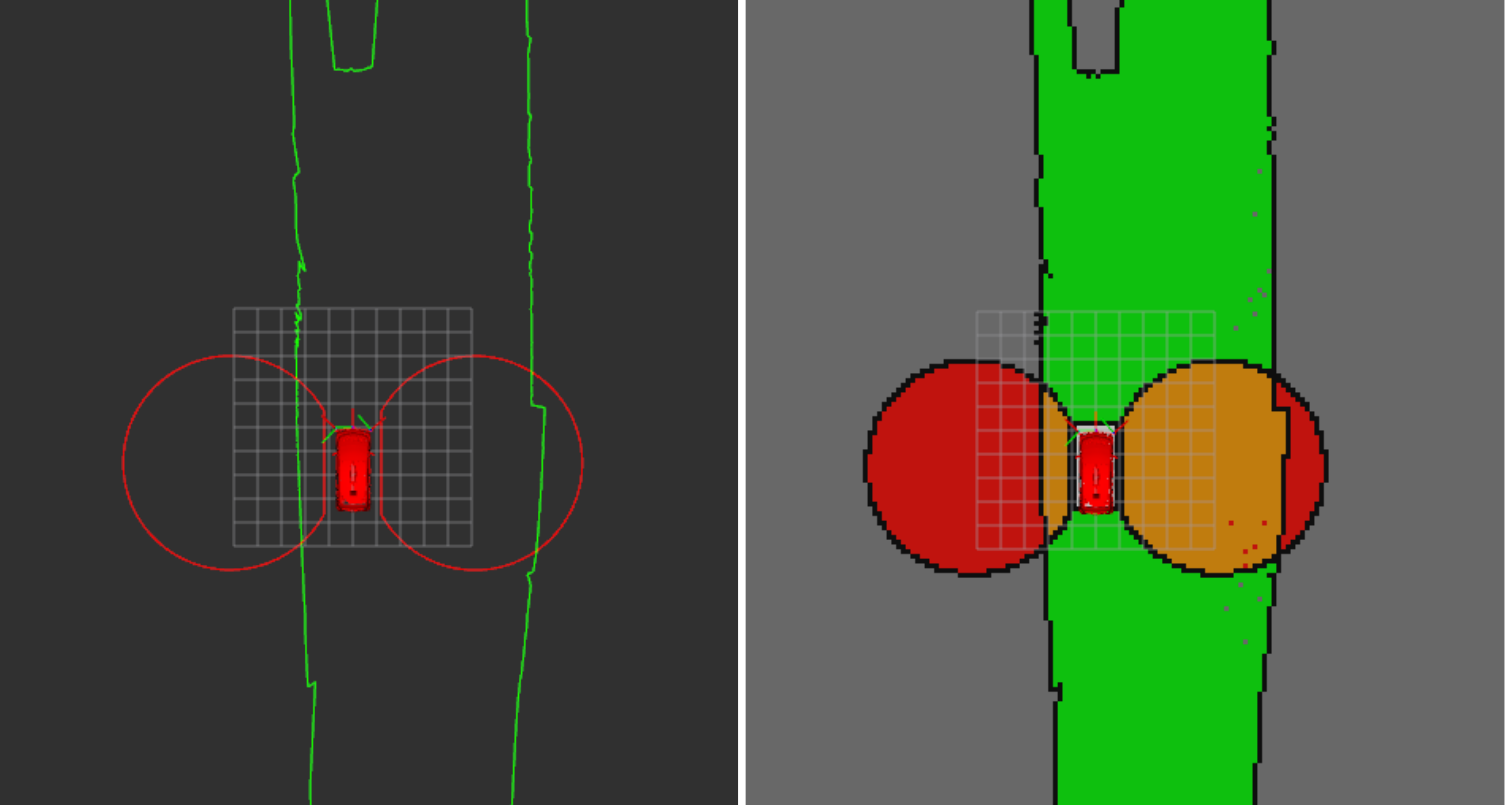
\includegraphics[width=1\textwidth]{capstate/imgs/diogo.png}
	
	\caption{Free space represented by a polygon (left) and an occupancy grid (right) (\cite{Correia2017})}
	\label{fig:diogo}
	
\end{figure}

\subsection{Active Tracking of Dynamic Multivariate Agents} 

Methods to detect and follow targets using the \gls{lidar} on the ATLASCAR were developed by  \cite{SoaresDeAlmeida2016a}. The thesis is based in the tracking of multiple targets in the fields of advanced safety systems. The focus lies in the prediction of the movement and actions of external agents. Two main targets are studied: vehicles and pedestrians. 

This thesis proposes techniques to improve motion prediction to achieve the development of algorithms capable of target tracking. These algorithms make use of the 3D point clouds of the environment and vision-based sensors. 

\section{ADAS Datasets - Examples of Labelled Data}

This sections presents some relevant work and its results in public labelled datasets for \gls{adas} projects.

\subsection{KITTI Dataset}
Probably the most well-known dataset in the fields of \gls{ad} is the \gls{kitti} (\cite{KarlsruheInstituteofTechnology}). The \gls{kitti} dataset was captured with a Volkswagen station wagon (figure \ref{fig:kitticar}) used in mobile robotics and \gls{ad} research. The \gls{kitti} benchmark suite started in 2012 at Karlsruhe Institute of Technology with the need to have a dataset to classify objects on the streets. 

This project has grown by increasingly adding more results with more sensors. The \gls{kitti} benchmark started with the stereo, flow and odometry benchmarks and today it includes standards for object tracking and more. 

\begin{figure}
	
	\centering
	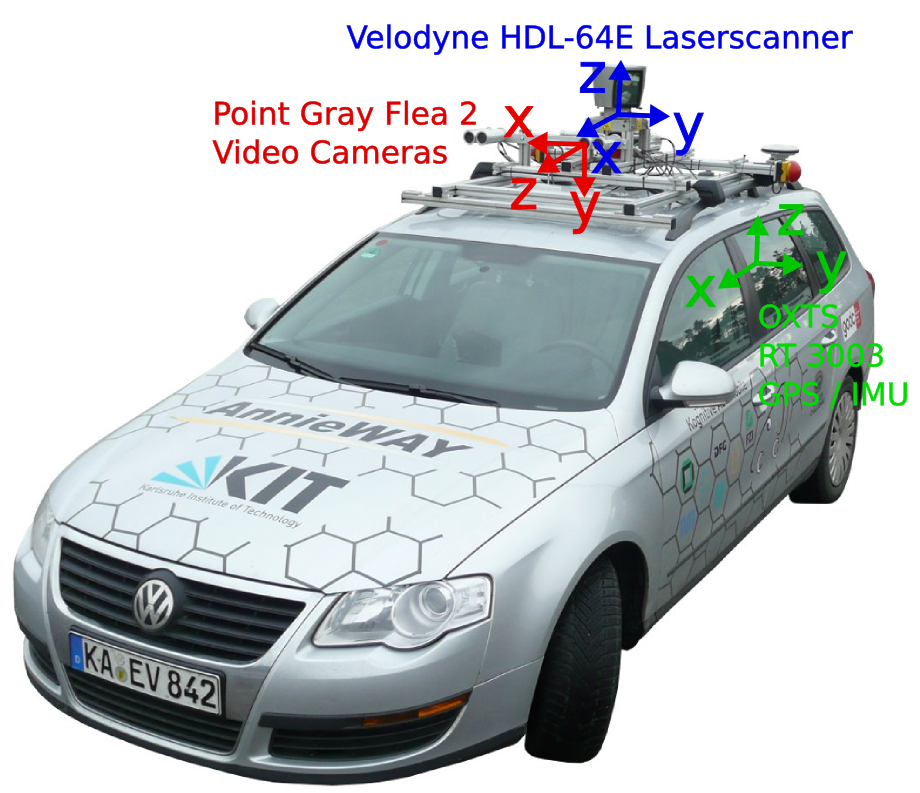
\includegraphics[width=0.6\textwidth]{capstate/imgs/kitticar}
	
	\caption{Volkswagen Station Wagon used in the KITTI Dataset (\cite{KarlsruheInstituteofTechnology})}
	\label{fig:kitticar}
	
\end{figure}

Just like ATLASCAR 2, the car used in the \gls{kitti} dataset is equipped with \gls{lidar} sensors and Point Grey Video Cameras. The dataset is used for automatic recognition and tracking of vehicles and pedestrians. 

It consists in image sequences (see figure \ref{fig:kittiresult}) and a text file in which, for each frame the various objects in the field of view are depicted with and identification number, a label, and coordinates about their position in the 2D and 3D space (\cite{Geiger}). 

The development kit used for the KITTI database contains C++ and MATLAB code to read the sensor data and write dataset results. The data development kit used is provided on the KITTI Website (\cite{KarlsruheInstituteofTechnology}). It contains a MATLAB demonstration code with C++ wrappers. 

The demonstration script of the KITTI development kit shows how 3D boxes can be read from the dataset files and projected into the image plane of the cameras (see figure \ref{fig:kittidk}). 

\begin{figure}[!hb]
	
	\centering
	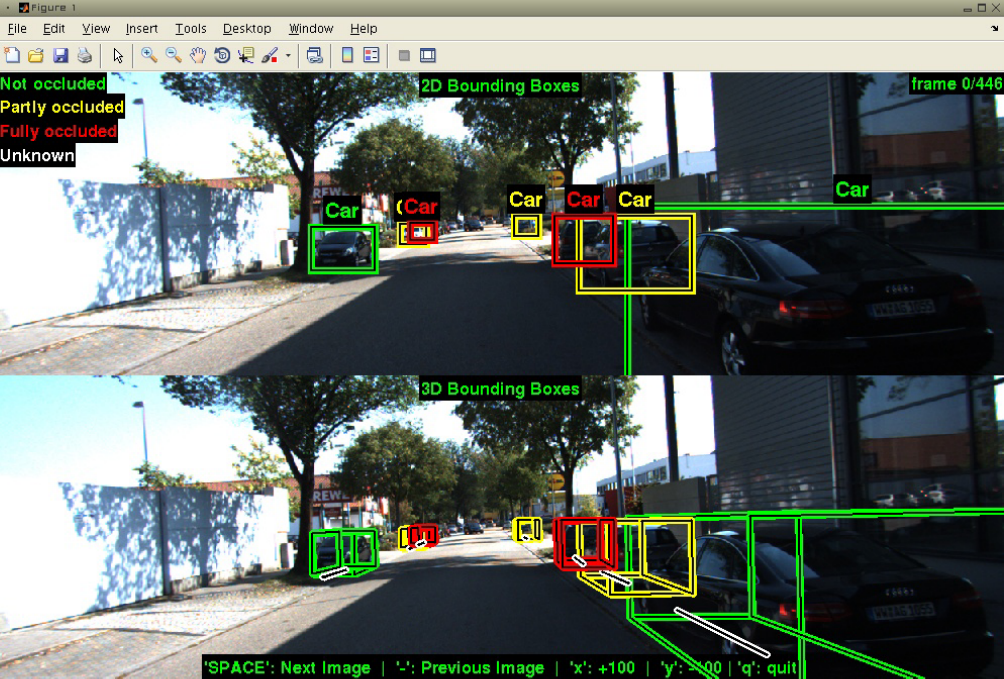
\includegraphics[width=0.85\textwidth]{capstate/imgs/kittidk.png}
	
	\caption{KITTI development kit showing 2D and 3D bounding boxes around several cars (\cite{KarlsruheInstituteofTechnology})}
	\label{fig:kittidk}
	
\end{figure}

The data is processed and inserted into MATLAB structures and arrays. The KITTI database also uses the \gls{pcl} to process and gather the pointclouds obtained from the LIDAR sensors.


\begin{figure}
\begin{center}
	\begin{lstlisting}[caption={KITTI dataset file snippet presenting frame\_id, object\_id, label, truncated and occluded flags, alpha, left top and right bottom coordinates, height, width and length, 3D coordinates (x,y,z) and rotation}, language=xml, label={lst: pop_grid}]
	...
	3 1 Cyclist 0 0 -1.931469 759.786603 146.098339 954.280160 374.000000 1.739063 0.824591 1.785241 1.821119 1.569936 5.783265 -1.642450
	3 2 Pedestrian 0 0 -2.547728 1154.836779 148.360923 1241.000000 321.627088 1.714062 0.767881 0.972283 6.463579 1.474131 7.560739 -1.860031
	4 -1 DontCare -1 -1 -10.000000 252.530000 168.660000 284.460000 202.850000 -1000.000000 -1000.000000 -1000.000000 -10.000000 -1.000000 -1.000000 -1.000000
	4 0 Van 0 0 -1.808333 290.287584 146.641981 444.387179 269.473545 2.000000 1.823255 4.433886 -4.934786 1.601945 14.098646 -2.139796
	4 1 Cyclist 0 0 -1.929519 767.158958 140.942948 961.992360 374.000000 1.739063 0.824591 1.785241 1.881359 1.534695 5.785600 -1.631447
	4 2 Pedestrian 1 0 -2.557045 1180.675035 151.025283 1241.000000 325.015204 1.714062 0.767881 0.972283 6.516488 1.497786 7.267796 -1.846627
	...	\end{lstlisting}
\end{center}
\end{figure}

Listing \ref{lst: pop_grid} shows an example snippet of what the \gls{kitti} dataset looks like. Each line starts with the frame ID and the ID of the object being tracked. Then it is added a label to classify this object. There are also flags to indicate if the object is either truncated or occluded in the image sequence. 

The following numbers consist in the alpha (observation angle of object), the left, top, right and bottom of the 2D bounding box, the height, width and length of the 3D bounding box and its XYZ coordinates. The last number consists in the 3D rotation angle in the Y axis (\cite{Team}).

Analyzing the snippet, a cyclist and a pedestrian can be located in frame 3 and the same cyclist and pedestrian (because they have the same object\_id) in the next frame with also a van. The \texttt{DontCare} label is often shown representing an object detected that is not related to the scope of the \gls{kitti} dataset. Other information indicate where these objects are found relatively to the car.

Figure \ref{fig:kittiresult} depicts a result from an image sequence using the KITTI dataset. 

\begin{figure}[h]
	
	\centering
	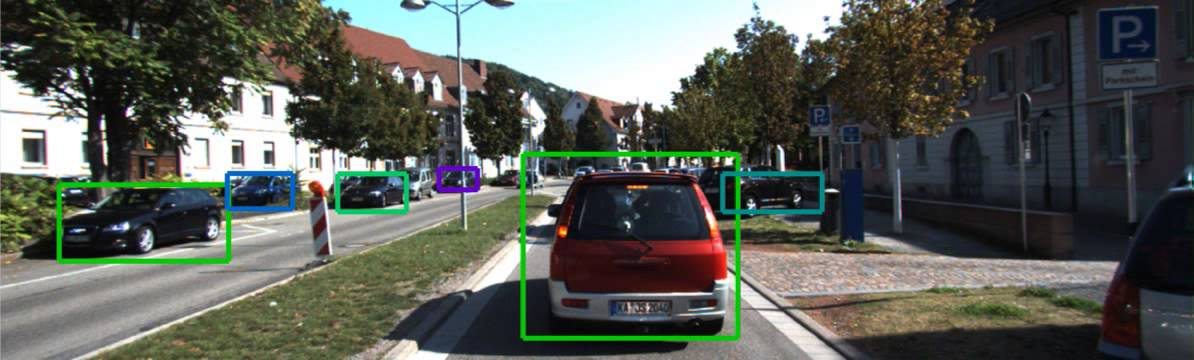
\includegraphics[width=0.99\textwidth]{capstate/imgs/kittiresult}
	
	\caption{Sequence example of tracking by detection using the \gls{kitti} dataset (\cite{KarlsruheInstituteofTechnology})}
	\label{fig:kittiresult}
	
\end{figure}

\subsection{Berkeley DeepDrive Dataset}

The DeepDrive Dataset is a recent \gls{adas} labelled dataset from the University of California, Berkeley.

The Dataset consists of box annotations, region annotations and detection of objects, lanes and drivable areas (\cite{Yu2018}). The only source data for each dataset is a video captured with a camera on a vehicle. Their labelling system is a web-based tool (see figure \ref{fig:berkeletool}). 

\begin{figure}[htp]
	
	\centering
	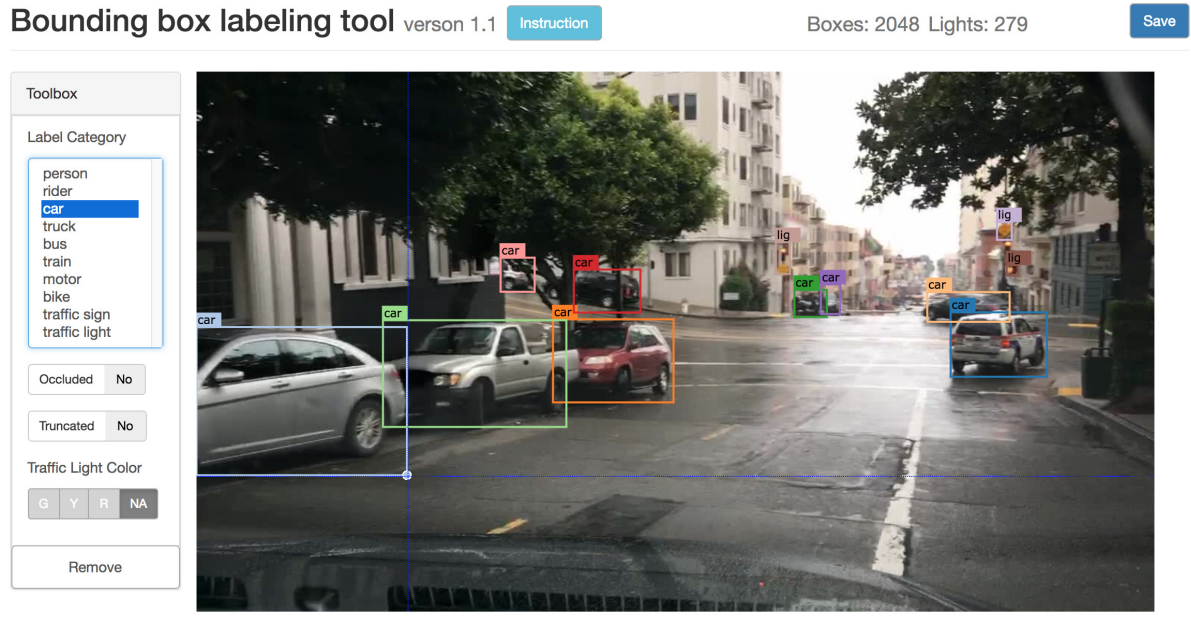
\includegraphics[width=0.99\textwidth]{capstate/imgs/berveleytool.png}
	
	\caption{DeepDrive Dataset Annotation Tool (\cite{Yu2018})}
	\label{fig:berkeletool}
	
\end{figure}

The labelling has a semi-automatic and a manual mode. In this annotation application the objects of interest are suggested with a bounding box and a category (label). The size of the bounding box and the category can be edited if the system fails. The objects are detected using a previously trained object detection model. 

\begin{figure}
	\begin{center}
		\begin{lstlisting}[label={lst:berkelydata}, caption={DeepDrive dataset file snippet.},language=C++]
		...
		    "frames": [
		    {
			    "timestamp": 10000,
			    "objects": [
			    {
				    "category": "car",
				    "id": 0,
				    "attributes": {
				    "occluded": true,
				    "truncated": false,
				    "trafficLightColor": "none"
				    },
				    "box2d": {
				    "x1": 555.647397,
				    "y1": 304.228432,
				    "x2": 574.015906,
				    "y2": 316.474104
				    }
			    },
			    {
				    "category": "car",
				    "id": 1,
				    "attributes": {
				    "occluded": true,
				    "truncated": false,
				    "trafficLightColor": "none"
				    },
				    "box2d": {
				    "x1": 554.116689,
				    "y1": 318.004813,
				    "x2": 567.89307,
				    "y2": 328.719775
				    }
		    },
		...	\end{lstlisting}
	\end{center}
\end{figure}

In listing \ref{lst:berkelydata} a snippet from a file of the DeepDrive dataset is depicted. The dataset is presented in the JSON format. For each frame there is a timestamp and a set of objects. Each object is identified with a category, an ID, attributes that indicate if the object is occluded, truncated, and if the object is a traffic light which light color is on. The position is represented by the 2D bounding box position $(x1,y1,x2,y2)$.

	
\subsection{HumanEva II Dataset}
The HumanEva II Dataset from the \gls{mpii} was also an interesting dataset, although it is used mainly for pedestrian detection.

This dataset appears with the need to represent information about detection and tracking of humans and their poses captured by a single image camera. The HumanEva dataset development kit includes several MATLAB modules, each one implementing a feature. Some modules refer to the body pose, others to image stream processing, writing the dataset results, and so on. Each script implements a chunk of the system that gathers the data and shapes it into MATLAB structures to be processed and to create the dataset.

The HumanEva dataset has information about the bounding boxes position used to track and detect pedestrian limb poses. This information is useful to know which direction the person is facing from the 3D skeleton derived from the pose. The data structure in the dataset is similar to a XML file. For each frame in the image sequences there are several bounding boxes with the respective coordinates (\cite{Sigal}).

\begin{figure}
\lstinputlisting[label={lst:humaneva_snip}, caption={HumanEva dataset file snippet.},language=xml]{capstate/files/humaneva_snip.xml}
\end{figure}

\begin{figure}[htp]
	
	\centering
	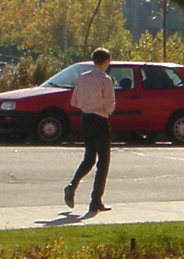
\includegraphics[width=0.5\textwidth]{capstate/imgs/00050.png}
	
	\caption{Example image of the HumanEva dataset that generated the snippet in listing \ref{lst:humaneva_snip} (\cite{Max-Planck-Gesellschaft}) }
	\label{fig:00050}
	
\end{figure}

By looking at listing \ref{lst:humaneva_snip}, in this dataset snippet is easy to identify the interest points in the given frame. The files are a set of annotations called $annotationList$ in which a path to the image corresponding to the frame is given. For each image there are several bounding boxes with coordinates $(x1,y1,x2,y2)$, a score, silhouette, articulation and viewpoint id.

\subsection{Other relevant datasets}
Other datasets included in the research for this dissertation are found in \gls{ethz} and in \gls{epfl} projects. 
\subsubsection{ETHZ dataset}
\gls{ethz} conducted studies for detection and tracking of people on the street (\cite{Ess2009}). Just like the previous datasets, its creation is based in MATLAB scripts and the data is gathered and stored in MATLAB structures. The dataset is simple: for each frame there are several bounding boxes in the image.
\begin{figure}
\begin{center}
	\begin{lstlisting}[label={lst:ETHZ}, caption={ETHZ dataset dataset file snippet (\cite{ETHZEidgenossischeTechnischeHochschuleZurich})},language=c++]
	...
	"left/image_00000015_0.png": (222, 177, 268, 312), (373, 105, 463, 393), (458, 220, 487, 285), (310, 225, 327, 265), (335, 228, 352, 264), (267, 228, 281, 261);
	"left/image_00000016_0.png": (220, 172, 266, 313), (378, 407, 476, 102), (462, 219, 486, 285), (312, 223, 327, 264), (337, 226, 352, 262), (267, 231, 279, 260);
	"left/image_00000017_0.png": (219, 173, 267, 316), (394, 94, 489, 423), (313, 222, 330, 262), (338, 227, 354, 262), (267, 228, 279, 260);
	...	\end{lstlisting}
\end{center}
\end{figure}

\begin{figure}[htp]
	
	\centering
	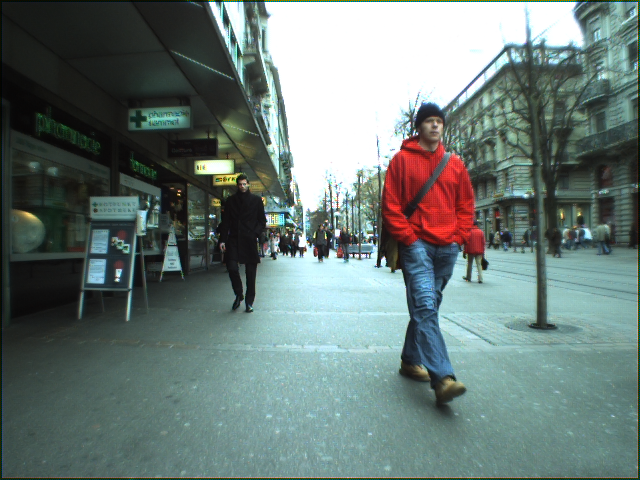
\includegraphics[width=0.7\textwidth]{capstate/imgs/image_00000016_0.png}
	
	\caption{One of the images of the \gls{ethz} dataset that generated part of the snippet in listing \ref{lst:ETHZ} (\cite{ETHZEidgenossischeTechnischeHochschuleZurich})}
	\label{fig:ETHZ}
	
\end{figure}

This dataset is focused only in the detection and tracking of pedestrians in the image (\cite{ETHZEidgenossischeTechnischeHochschuleZurich}). In listing \ref{lst:ETHZ} each line is composed with a string defining a path to the image representing the actual frame, followed by tuples of four elements $(x1,y1,x2,y2)$ representing the bounding boxes where pedestrians are found in the respective frame. 

\subsubsection{EPFL dataset}
The \gls{epfl} designed a dataset for multiple people in a camera environment, independent of the scenario. This dataset used various synced video cameras filming the same area in different angles (\cite{Biliotti}). The data from the cameras is captured and processed with MATLAB scripts and some algorithms in C++.

\begin{figure}
\begin{center}
	\begin{lstlisting}[label={lst:basket}, caption={EPFL dataset file snippet (\cite{EPFLEcolepolytechniquefederaledeLausanne})},language=c++]
									...
									1 80 45 99 98 9363 0 0 1 "PERSON"
									1 80 45 99 98 9364 0 0 0 "PERSON"
									1 77 45 96 98 9365 0 0 1 "PERSON"
									1 74 45 93 98 9366 0 0 1 "PERSON"
									1 71 46 90 99 9367 0 0 0 "PERSON"
									2 81 45 110 126 0 0 0 0 "PERSON"
									2 80 45 109 126 1 0 0 1 "PERSON"
									2 80 45 109 126 2 0 0 1 "PERSON"
									2 80 45 109 126 3 0 0 1 "PERSON"
									2 80 45 109 126 4 0 0 1 "PERSON"
									...	\end{lstlisting}
\end{center}
\end{figure}

\begin{figure}[htp]
	
	\centering
	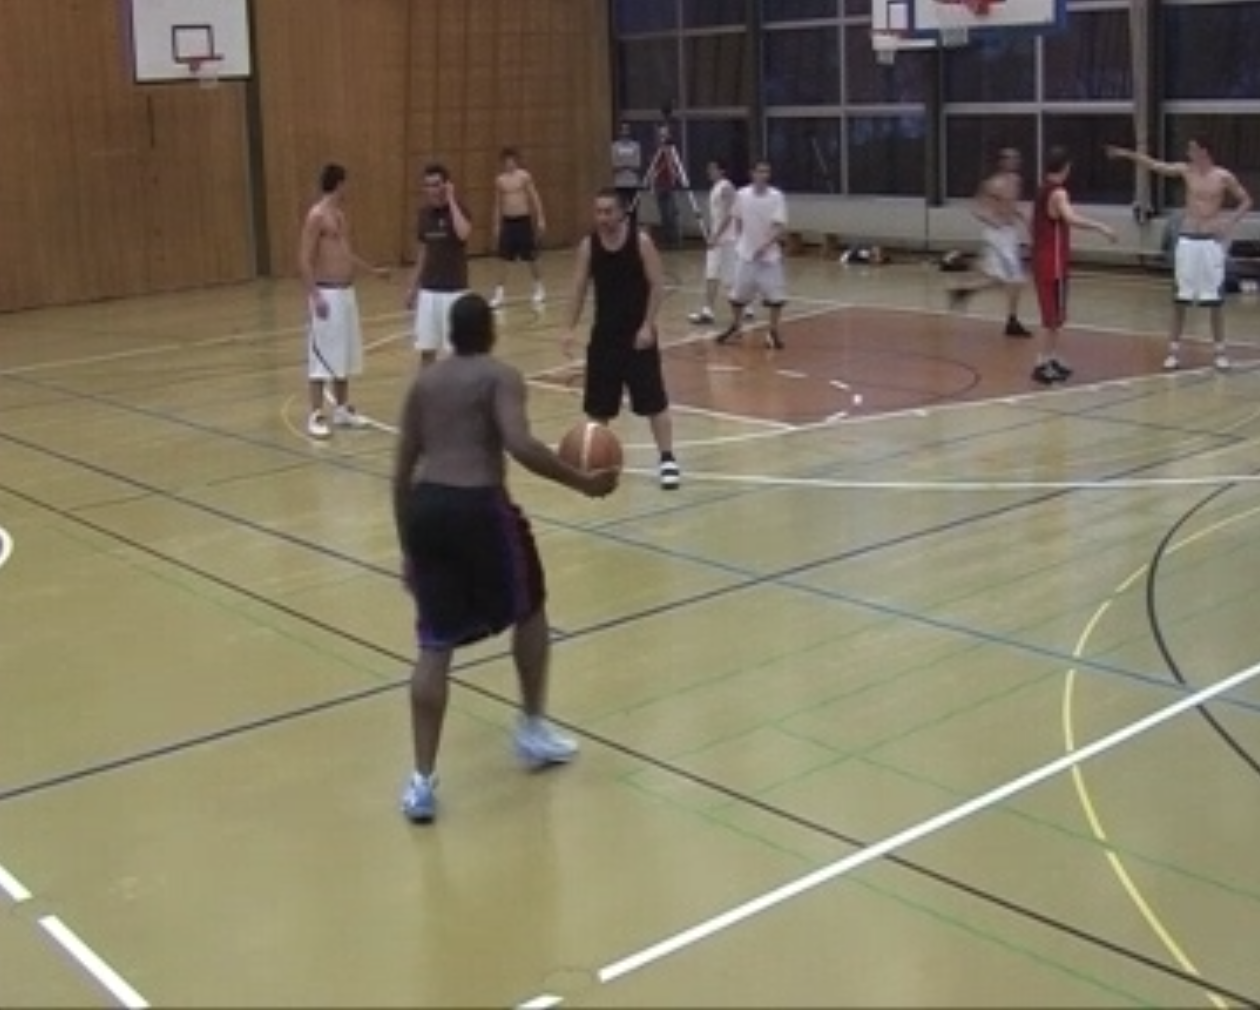
\includegraphics[width=0.7\textwidth]{capstate/imgs/basket.png}
	
	\caption{One of the images of the \gls{epfl} dataset that generated part of the snippet in listing \ref{lst:basket} (\cite{EPFLEcolepolytechniquefederaledeLausanne})}
	\label{fig:basketimg}
	
\end{figure}


In listing \ref{lst:basket} there is a snippet of the dataset. The dataset includes, for each frame, various objects identified with a number, a label, bounding box coordinates, and flags to point out if the person is occluded, lost, or if the detection was automatically interpolated from the other camera's information (\cite{EPFLEcolepolytechniquefederaledeLausanne}). The particularity of the structure of this dataset is that, for each object, it is tracked in the image sequences individually, and only then another object is tracked and labeled. In listing \ref{lst:basket_leg} a legend of this dataset can be found.

\begin{figure}[htp]

\begin{center}
	\begin{lstlisting}[label={lst:basket_leg}, caption={EPFL dataset legend.}]
	track_id. All rows with the same ID belong to the same path
	xmin. The top left x-coordinate of the bounding box
	ymin. The top left y-coordinate of the bounding box
	xmax. The bottom right x-coordinate of the bounding box
	ymax. The bottom right y-coordinate of the bounding box
	frame_number. The frame that the annotation represents
	lost. If 1, the annotation is outside of the view screen
	occluded. If 1, the annotation is occluded
	generated. If 1, the annotation was automatically interpolated
	label. (human, car/vehicle, bicycle...)	\end{lstlisting}
\end{center}

\end{figure}
 
\subsection{Resume}

To summarize this section, after analyzing these datasets and how they are created, it is important to look at what is stored in the data structures	. Some datasets use well known data structures such as XML (HumanEva) or JSON (DeepDrive), and some datasets use their own set of data where each line corresponds to an entry. 

To design a dataset for the ATLASCAR it is necessary to decide which construction to use. To simplify the complexity of the files, an adapted approach used in the KITTI dataset will be used, where each line is an entry for a different object.

Analyzing the datasets, the most common and relevant information in all files is the position of the targets, their classification and identification. So it is fundamental for the ATLASCAR dataset to contain, for each frame, 2D and 3D coordinates of the target, a label, and an identification number.

Regarding the labelling system, it would be interesting to implement an interface that suggests the user objects of interest similar to the DeepDrive annotation tool.



